% CVPR 2024 Paper Template; see https://github.com/cvpr-org/author-kit

\documentclass[10pt,twocolumn,letterpaper]{article}
\usepackage{kotex}

%%%%%%%%% PAPER TYPE  - PLEASE UPDATE FOR FINAL VERSION
 \usepackage{cvpr}              % To produce the CAMERA-READY version
%\usepackage[review]{cvpr}      % To produce the REVIEW version
% \usepackage[pagenumbers]{cvpr} % To force page numbers, e.g. for an arXiv version

% Import additional packages in the preamble file, before hyperref
%
% --- inline annotations
%
\usepackage[dvipsnames]{xcolor}
\newcommand{\red}[1]{{\color{red}#1}}
\newcommand{\todo}[1]{{\color{red}#1}}
\newcommand{\TODO}[1]{\textbf{\color{red}[TODO: #1]}}
% --- disable by uncommenting  
% \renewcommand{\TODO}[1]{}
% \renewcommand{\todo}[1]{#1}



% It is strongly recommended to use hyperref, especially for the review version.
% hyperref with option pagebackref eases the reviewers' job.
% Please disable hyperref *only* if you encounter grave issues, 
% e.g. with the file validation for the camera-ready version.
%
% If you comment hyperref and then uncomment it, you should delete *.aux before re-running LaTeX.
% (Or just hit 'q' on the first LaTeX run, let it finish, and you should be clear).
\definecolor{cvprblue}{rgb}{0.21,0.49,0.74}
\usepackage[pagebackref,breaklinks,colorlinks,citecolor=cvprblue]{hyperref}

%%%%%%%%% PAPER ID  - PLEASE UPDATE
\def\paperID{010} % *** Enter the Paper ID here
\def\confName{CVPR}
\def\confYear{2024}

%%%%%%%%% TITLE - PLEASE UPDATE
\title{Computer Vision Final Team Project}

%%%%%%%%% AUTHORS - PLEASE UPDATE
\author{Seongho Jeong
\\Yonsei University
{\tt\small seongho79.jeong@yonsei.ac.kr}
% For a paper whose authors are all at the same institution,
% omit the following lines up until the closing ``}''.
% Additional authors and addresses can be added with ``\and'',
% just like the second author.
% To save space, use either the email address or home page, not both
\and
Gwangil Choi
\\Yonsei University
{\tt\small 	gwangil.choi@yonsei.ac.kr}
}

\begin{document}
\maketitle
\begin{abstract}
실제 배포 환경에서는 학습(source)-배포(target) 간 도메인 편차로 인해 모델 성능이 급격히 저하된다. 본 연구는 이러한 문제를 해결하기 위해 통계적 정렬 기반 MMD, 주파수 증강 기반 FACT, Cosine Similarity 정렬 손실, 그리고 위상 지터와 그래프 일관성을 결합한 신규 기법 FPJ-GC를 ResNet-50 기반 분류기에 적용해 비교하였다. PACS 데이터셋으로 학습하고 동일 카테고리의 실사 이미지를 수집해 구축한 CuratedPACS로 성능을 평가한 결과, 기존 베이스라인(69.40 / 66.53) 대비 FACT(+11.5 \~ 10.7), Cosine Similarity(+12.0 \~ 12.3), FPJ-GC(+12.4 \~ 15.6)가 일관된 정확도 향상을 보였다. 특히 FPJ-GC는 추가 파라미터 없이 위상 기반 변형과 배치 전역 그래프 정합성을 동시에 활용해 가장 높은 평균 정확도(81.83 / 82.09)와 낮은 성능 분산을 기록했다.

\end{abstract}    
\section{Introduction}
\label{sec:intro}

최근 딥러닝 모델은 대규모 데이터에 기반해 뛰어난 성능을 달성하고 있지만, 
훈련(Source) 환경과 배포(Target) 환경 사이의 도메인 편차(Domain Shift)가 존재할 때 
성능이 급격히 저하되는 한계를 드러낸다. 이러한 문제를 해결하고자 제안된 Task가 바로 
도메인 일반화(Domain Generalization, DG) 이며, 해당 task 는 학습 단계에서 접하지 
않은 도메인에서도 일관된 성능을 유지하는 표현을 학습하는 것을 목적으로 하며 본 
보고서에서는 과제에서 제시한것중 세가지 방법과, 새로 아이디어를 낸 세가지 방법을 
비교하였다.

\subsection{과제에서 제시한 방법}
\begin{enumerate}[leftmargin=2em]
  \item ResNet-50 기반 Baseline
  \item 통계적 정렬 계열 기법인 MMD
  \item 주파수 기반 증강 기법인 FACT
\end{enumerate}

\subsection{새로운 아이디어를 더한 방법}
\begin{enumerate}[leftmargin=2em]
  \item MMD + Cosine Similarity 정렬 손실
  \item FPJ-GC : Fourier‑Phase Jitter with Graph Consistency
  \item LaPaR : Latent‑Patch Re‑Masking
\end{enumerate}

각 방법의 이론적 배경과 구현 세부를 설명하고, PACS 데이터셋 및 비공개 Real 도메인에서의 
실험 결과를 통해 제안 기법의 우수성과 안정성을 검증하는 것을 목표로 한다.

%-------------------------------------------------------------------------
\section{Related Works}
해당 섹션에서는 Final Project에서 Reference로 주어진 Base Code과 두가지 일반화 방법에 대해서 설명하고자 한다.
\vspace{1em}
\begin{itemize}[leftmargin=2em]
  \item \textbf{BASE} \cite{he2016residual}:{“implements a ResNet50 model trained on the PACS dataset using standard cross-entropy loss”}
  \item \textbf{MMD} \cite{muandet2013invariant}:{“Domain Generalization via Invariant Feature Representation”}
  \item \textbf{FACT} \cite{xu2021fact}:{“A Fourier-based Framework for Domain Generalization”}
\end{itemize}

\subsection{Base Code}
..

\begin{figure}[h]
  \centering
  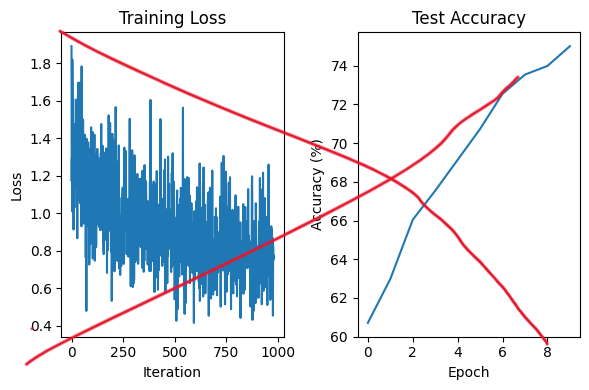
\includegraphics[width=\linewidth]{images/temp.png}
  \caption{Base Line}
  \label{fig:BASE1}
\end{figure}

\subsection{MMD}
Team project reference 논문 중 하나인 “Domain Generalization via Invariant 
Feature Representation” 의 일반화 방법이며 도메인 간 Global Alignment 를 잘 수행하여 각 
객체에 대한 Invariant Feature Representation 을 획득해 일반화를 수행하는 것을 목표로 한다.

\subsubsection{Main Idea}
서로 다른 소스 도메인들의 Feature Distribution 을 Kernel Space 에서 일치시키게 된다면, 
보지 못한 도메인에서도 분포가 크게 어긋나지 않아 모델이 Instance 에 대한 Invariant Feature 
Representation 학습하게 된다.

\subsubsection{Method}
기존 Kernel Space 의 Feature 를 Gaussian Kernel 로 Mapping 하여 Mean 
Embedding 을 구하고 모든 도메인 쌍에 대해 차를 합산. 이를 이용하여 두 Feature Distribution을 
일치시키는 방법론이다.

\begin{figure}[h]
  \centering
  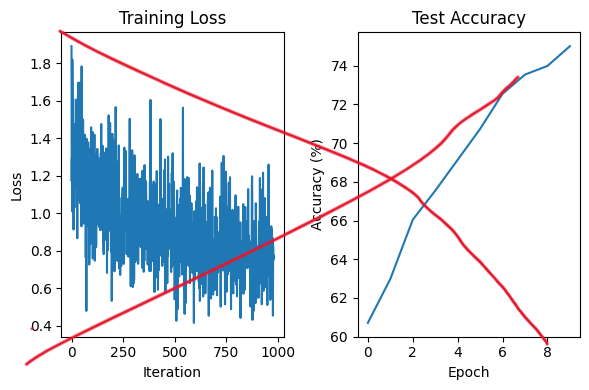
\includegraphics[width=\linewidth]{images/temp.png}
  \caption{MMD}
  \label{fig:MMD1}
\end{figure}

\subsection{FACT}
Final Team Project Reference 논문 중 하나인 “A Fourier-based Framework for Domain 
Generalization” 의 일반화 방법이며 저주파 진폭은 도메인 특유의 정보를 많이 담고있다는 걸 이용하여 
저주파 진폭에 대한 가짜 도메인을 FFT 를 통해 증강하여 네트워크가 저주파 진폭에 대한 의존도를 줄이고 
위상에 대한 의존도를 높이게끔 유도하여 Invariant Representation 을 습득하고자 하는 방법론이다.

\subsubsection{Main Idea}
이미지의 위상 (Phase) 는 고차원적인 의미를 담고, 저주파 진폭 (Low-freq Amplitude) 는 
도메인의 조명, 스타일 같은 각 도메인 특유의 정보가 많다. 따라서, 이런 특성을 지닌 저주파 진폭을 
섞어 가짜 도메인을 만들어 네트워크에 Perturbation 을 주게 된다면 도메인 특유에 대한 정보에 노이즈가 
심해져 의존도가 기존보다 줄어 들고 객체의 형태나 고유 정보를 포함하고 있는 위상정보에 더 의존하게 
되는 Invariant Representation 을 학습할 수 있다.

\subsubsection{Method}
두 이미지를 Fast Fourier Transform (FFT) 로 분해하여 진폭과 위상을 분리하여 저주파 영역에 
선형보간을 수행해 Amplitude 에 Mix 을 수행한다. 이후, iFFT 를 통해 공간 도메인을 복원하고 
Student/Teacher 에 동시 입력하여 원본과 Mix 간 이미지 예측값이 모두 일관되도록 수행한다.

\begin{figure}[h]
  \centering
  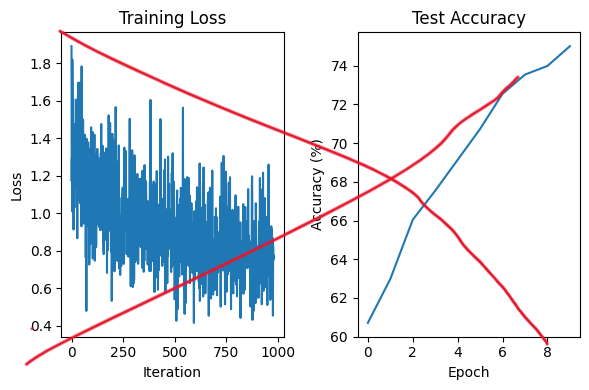
\includegraphics[width=\linewidth]{images/temp.png}
  \caption{FACT}
  \label{fig:FACT1}
\end{figure}

%-------------------------------------------------------------------------

\section{Proposed methods}
해당 섹션에서는 우리가 제안하는 방법론인 아래 세가지 방법에 대해서 설명하고자 한다.
\vspace{1em}
\begin{itemize}[leftmargin=2em]
  \item MMD-Cos : MMD + Cosine Similarity
  \item FPJ-GC : Fourier‑Phase Jitter with Graph Consistency
  \item LaPaR : Latent‑Patch Re‑Masking
\end{itemize}

\subsection{MMD-Cos}

기존 MMD 는 Gaussian Kernel 을 통해 변환된 Feature 를 서로 근사시키는데 반해, 
해당 방법은 Gaussian Kernel 을 Cosine Simiarity 로 바꿈으로써 Gaussian Kernel의 
Hyper Parameter Choice 에서도 자유롭고, 직접적으로 벡터의 방향만 비교함으로써 
같은 클래스들을 도메인과 관계없이 보다 잘 정렬시켜 일반화 능력을 강화한다.

\subsubsection{Method}
Gaussian Kernel 을 Cosine Similarity 로 변환하여 MMD 를 수행한다.

\begin{figure}[h]
  \centering
  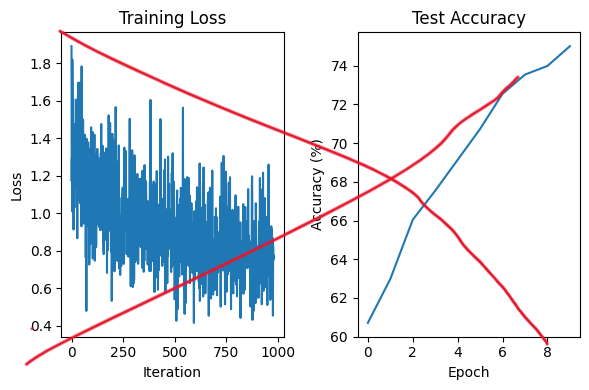
\includegraphics[width=\linewidth]{images/temp.png}
  \caption{MMD-Cos}
  \label{fig:MMD-Cos1}
\end{figure}

\subsection{FPJ-GC}
Phase 스펙트럼에 저/고주파별 미세 노이즈를 가해 Style-invariant 구조 
변형을 만들고, 원본 배치와 Jitter 배치가 동일한 Cosine Simialrity Graph를 
유지하도록 학습하게 됨으로써 도메인 변화에 보다 강인한 Feature 를 획득하게끔하는 방법론이다.

\subsubsection{Main Idea}
Amplitude (FACT, Mix-style) 과 달리 phase 를 조작하며 개별 샘플 일치 대신 
배치-전역 그래프 일관성으로 보다 안정적으로 수렴하게 하여 강인한 feature를 획득하여 
일반화 능력을 강화한다.

\subsubsection{Pros}
Phase 중심 변조를 통해 shape-shift 도메인에 강하고 배치레벨 그래프를 통해 개별 
alignment 보다 안정적이게 되면서 자연스레 collapse 위험도가 낮게 되고, 기존 방식들에서 
추가적인 parameter 를 요구하지 않기에 computation cost 증가에서 자유롭다.

\subsubsection{Differences from Existing Methodologies}
amplitude 변환을 통해 도메인에 대한 정보 의존도를 줄여 일반화 능력을 강화하는 기존의 
방식들과 다르게, phase jitter 를 통해 보다 robust 한 특성을 직접적으로 습득하면서 
Graph consistency 를 원본과 변형의 관계 유지용으로 사용하기에 기존 연구와의 차이가 있다.

\begin{figure}[h]
  \centering
  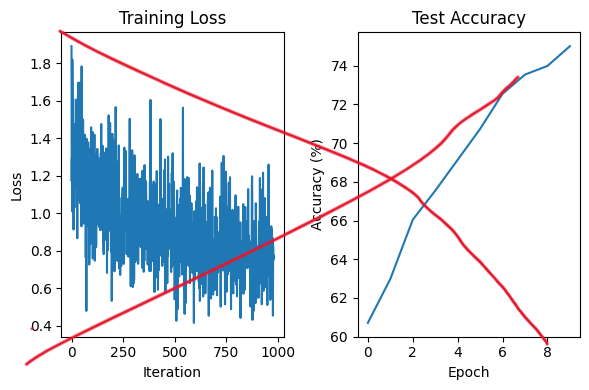
\includegraphics[width=\linewidth]{images/temp.png}
  \caption{FPJ-GC}
  \label{fig:FPJ-GC1}
\end{figure}

\subsection{LaPaR}
분석 내용 작성 예정\\
분석 내용 작성 예정\\
분석 내용 작성 예정\\
분석 내용 작성 예정\\
분석 내용 작성 예정\\

\subsubsection{Main Idea}
분석 내용 작성 예정\\
분석 내용 작성 예정\\
분석 내용 작성 예정\\
분석 내용 작성 예정\\
분석 내용 작성 예정\\

\subsubsection{Pros}
분석 내용 작성 예정\\
분석 내용 작성 예정\\
분석 내용 작성 예정\\
분석 내용 작성 예정\\
분석 내용 작성 예정\\

\subsubsection{Differences from existing methodologies}
분석 내용 작성 예정\\
분석 내용 작성 예정\\
분석 내용 작성 예정\\
분석 내용 작성 예정\\
분석 내용 작성 예정\\

\begin{figure}[h]
  \centering
  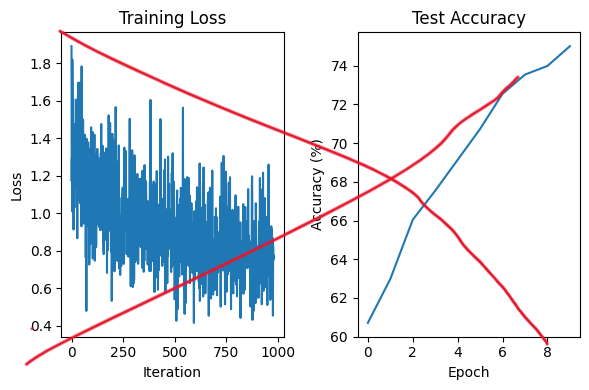
\includegraphics[width=\linewidth]{images/temp.png}
  \caption{LaPaR}
  \label{fig:LaPaR1}
\end{figure}

%-------------------------------------------------------------------------

\section{Experimental Results}
해당 섹션은 위에서 설명한 방법론들과 base 모델 간 비교를 통해 성능비교를 수행한다. 

\subsubsection{Experimental Environment}
\subsubsection{Baseline}
assignment 기본 설정에서 어떠한 변화를 주지 않고 classification 을 수행하며, 이후 실험 
또한 추가되는 방법에 대한 모듈을 제외한 모든 실험 환경은 baseline 과 동일하다.

\subsubsection{Method module config}
\begin{alltt}
MMD : sigma = (1, 2, 4, 8), lambda = 0.1
FACT : eta = 0.3, beta = 0.25, 
       temperature= 3.0 
MMD-Cos : lambda = 1.0
FPJ-GC : lambda graph = 0.2
\end{alltt}

\subsubsection{Dataset}
학습에는 기존 실험세팅에서 주어진 pre-trained weight 와 PACS dataset 을 사용했으나, test 셋은 PACS와 
동일한 카테고리를 지닌 실제 이미지들을 크롤링하여 50장씩 구성한 CuratedPACS 를 따로 구축하여 
성능비교 데이터셋으로 사용함. 

\subsection{Results}
\subsubsection{Base Code}
분석 내용 작성 예정\\
분석 내용 작성 예정\\
분석 내용 작성 예정\\
분석 내용 작성 예정\\
분석 내용 작성 예정\\
\begin{table}[h]
  \centering
  \begin{tabular}{lrrr}
  \toprule
  Iterations & Training & Test \\
  \midrule
  1 & -\% & -\% \\
  2 & -\% & -\% \\
  3 & -\% & -\% \\
  \bottomrule
  \end{tabular}
  \caption{Base Code: Results from 3 Experimental Iterations}
  \label{tab:Base Code: Results from 3 Experimental Iterations}
\end{table}

\subsubsection{MMD}
분석 내용 작성 예정\\
분석 내용 작성 예정\\
분석 내용 작성 예정\\
분석 내용 작성 예정\\
분석 내용 작성 예정\\
\begin{table}[h]
  \centering
  \begin{tabular}{lrrr}
  \toprule
  Iterations & Training & Test \\
  \midrule
  1 & -\% & -\% \\
  2 & -\% & -\% \\
  3 & -\% & -\% \\
  \bottomrule
  \end{tabular}
  \caption{MMD: Results from 3 Experimental Iterations}
  \label{tab:MMD: Results from 3 Experimental Iterations}
\end{table}

\subsubsection{FACT}
분석 내용 작성 예정\\
분석 내용 작성 예정\\
분석 내용 작성 예정\\
분석 내용 작성 예정\\
분석 내용 작성 예정\\
\begin{table}[h]
  \centering
  \begin{tabular}{lrrr}
  \toprule
  Iterations & Training & Test \\
  \midrule
  1 & -\% & -\% \\
  2 & -\% & -\% \\
  3 & -\% & -\% \\
  \bottomrule
  \end{tabular}
  \caption{FACT: Results from 3 Experimental Iterations}
  \label{tab:FACT: Results from 3 Experimental Iterations}
\end{table}

\subsubsection{MMD-Cos}
분석 내용 작성 예정\\
분석 내용 작성 예정\\
분석 내용 작성 예정\\
분석 내용 작성 예정\\
분석 내용 작성 예정\\
\begin{table}[h]
  \centering
  \begin{tabular}{lrrr}
  \toprule
  Iterations & Training & Test \\
  \midrule
  1 & -\% & -\% \\
  2 & -\% & -\% \\
  3 & -\% & -\% \\
  \bottomrule
  \end{tabular}
  \caption{MMD-Cos: Results from 3 Experimental Iterations}
  \label{tab:MMD-Cos: Results from 3 Experimental Iterations}
\end{table}

\subsubsection{FPG-GC}
분석 내용 작성 예정\\
분석 내용 작성 예정\\
분석 내용 작성 예정\\
분석 내용 작성 예정\\
분석 내용 작성 예정\\
\begin{table}[h]
  \centering
  \begin{tabular}{lrrr}
  \toprule
  Iterations & Training & Test \\
  \midrule
  1 & -\% & -\% \\
  2 & -\% & -\% \\
  3 & -\% & -\% \\
  \bottomrule
  \end{tabular}
  \caption{FPG-GC: Results from 3 Experimental Iterations}
  \label{tab:FPG-GC: Results from 3 Experimental Iterations}
\end{table}

\subsubsection{LaPaR}
분석 내용 작성 예정\\
분석 내용 작성 예정\\
분석 내용 작성 예정\\
분석 내용 작성 예정\\
분석 내용 작성 예정\\
\begin{table}[h]
  \centering
  \begin{tabular}{lrrr}
  \toprule
  Iterations & Training & Test \\
  \midrule
  1 & -\% & -\% \\
  2 & -\% & -\% \\
  3 & -\% & -\% \\
  Avg. & -\% & -\% \\
  \bottomrule
  \end{tabular}
  \caption{LaPaR: Results from 3 Experimental Iterations}
  \label{tab:LaPaR: Results from 3 Experimental Iterations}
\end{table}

\subsection{Analysis}
분석 내용 작성 예정\\
분석 내용 작성 예정\\
분석 내용 작성 예정\\
분석 내용 작성 예정\\
분석 내용 작성 예정\\
\begin{table}[h]
  \centering
  \begin{tabular}{lrr}
    \toprule
    & \multicolumn{2}{c}{Average Accuracy}\\
    \cmidrule(r){2-3}
    Model & Training & Test\\
    \midrule
    Base Code & -\% & -\%\\
    MMD & -\% & -\%\\
    FACT & -\% & -\%\\
    MMD-Cos & -\% & -\%\\
    FPG-GC & -\% & -\%\\
    LaPaR & -\% & -\%\\
    \bottomrule
  \end{tabular}
  \caption{Final Results about all models}
  \label{tab:Final Results about all models}
\end{table}


모든 제안 기법이 Baseline 대비 일관된 성능 향상을 달성하였다. 다만 다음 세 가지 실험적 제약을 고려할 필요가 있다.

\begin{enumerate}
  \item Curated PACS 표본 수의 한계 : 평가 세트가 작아 통계적 신뢰 구간이 넓다.
  \item PACS 자체의 소규모 규모 : 도메인 다양성이 제한적이어서 실제 배포 환경 전체를 대표하기 어렵다.
  \item 10 epoch로 제한된 학습 스케줄 : 충분한 수렴 이전 단계에서 모델 간 격차가 과소·과대평가될 수 있다.
\end{enumerate}

따라서 이번 결과를 절대적인 일반화 능력 차이로 단정하긴 이르다. 그럼에도 동일한 조건에서 관찰된 유의미한 우위는 
제안 기법들이 도메인 일반화에 실질적 효과가 있음을 강하게 시사한다. 더 큰 데이터셋과 장기 학습을 수행하게 된다면 
보다 안정화된 데이터를 얻을 수 있을 것으로 보여진다.

%-------------------------------------------------------------------------

\section{Concluding Remarks}
\subsection{실험을 여러번 돌린 이유}
단일 실행으로는 결과 해석이 어렵다는 사실이 초기 탐색에서 드러났다.
예를 들어 MMD 모델은 동일한 조건에서 시드만 달라졌을 때 정확도가 10 \%p 이상 변동했다. 
이런 편차가 존재하면, 새 모듈이 가져온 성능 변화가 실제 일반화 효과인지, 아니면 훈련 
불안정성 때문인지 구분하기 힘들다.\\
우리는 변동 원인으로 Color Jitter 등은 매 미니배치마다 다른 색 공간 변형을 주어 
일반화에 도움을 주지만, 증강 분산을 모델이 충분히 흡수·평균화하기엔 학습 시간이 짧기에 
증강 편차가 그대로 최종 성능의 노이즈로써 남게되는 것으로 추측하였다.\\
이에 대한 해결책으로 증강 시드 고정을 검토했으나 모델에 편향성을 학습시킬 위험과 과제에서 제시한 
기본 설정을 변경하게 되므로 실험에 영향을 줄 수 있기에 채택하지 않았다. 다른 방법으로 
우리는 여러번의 실험을 통해 평균적인 모델 성능을 구하여 방법론 자체가 가져온 효과를 보다 
신뢰성 있게 평가하는 방식을 선택했다.

\subsection{FPJ-GC 모델 선정 이유}
Curated PACS 평가에서는 Cosine Similarity와 FPJ-GC가 모두 높은 정확도를 보였다. 
그러나 Cosine Similarity 모듈은 MMD 효과를 강화하려고 유사도 손실 가중치(λ)를 높여야만성능이 극대화됐다. 
이 과정에서 하이퍼 파라미터에 대한 민감도가 증가하여 재현성이 떨어질 수 있다는 점과 성능 변동의 폭이 
FPJ-GC가 보다 작았으며 추가조정 또한 없었다는 점을 들어 최종선택을 하게 되었다.

\section{Conclusion}
본 과제의 목표는 Baseline 대비 도메인 일반화 성능을 향상시키면서도, 모델 구조나 계산 비용을 거의 늘리지 
않는 방법을 찾는 것이었다. 실험 결과 FPJ-GC모듈이 이 요구를 가장 잘 충족했다. 따라서 FPJ-GC는 이론적 타당성과 일반화 
성능을 모두 갖춘, 효과적인 도메인 일반화 솔루션으로 판단되어지며, 해당 모델을 우리들의 제안 모델로 선정하였다.


%
\begin{thebibliography}{9}
\bibitem{muandet2013}
Muandet \textit{et al.}, “Domain Generalization via Invariant Feature Representation,” ICML, 2013.

\bibitem{xu2021}
Xu \textit{et al.}, “A Fourier‐Based Framework for Domain Generalization,” CVPR, 2021.
\end{thebibliography}
%\section{Final copy}

You must include your signed IEEE copyright release form when you submit your finished paper.
We MUST have this form before your paper can be published in the proceedings.

Please direct any questions to the production editor in charge of these proceedings at the IEEE Computer Society Press:
\url{https://www.computer.org/about/contact}.
{
    \small
    \bibliographystyle{ieeenat_fullname}
    \bibliography{main}
}

% WARNING: do not forget to delete the supplementary pages from your submission 
% \clearpage
\setcounter{page}{1}
\maketitlesupplementary


\section{Rationale}
\label{sec:rationale}
% 
Having the supplementary compiled together with the main paper means that:
% 
\begin{itemize}
\item The supplementary can back-reference sections of the main paper, for example, we can refer to \cref{sec:intro};
\item The main paper can forward reference sub-sections within the supplementary explicitly (e.g. referring to a particular experiment); 
\item When submitted to arXiv, the supplementary will already included at the end of the paper.
\end{itemize}
% 
To split the supplementary pages from the main paper, you can use \href{https://support.apple.com/en-ca/guide/preview/prvw11793/mac#:~:text=Delete%20a%20page%20from%20a,or%20choose%20Edit%20%3E%20Delete).}{Preview (on macOS)}, \href{https://www.adobe.com/acrobat/how-to/delete-pages-from-pdf.html#:~:text=Choose%20%E2%80%9CTools%E2%80%9D%20%3E%20%E2%80%9COrganize,or%20pages%20from%20the%20file.}{Adobe Acrobat} (on all OSs), as well as \href{https://superuser.com/questions/517986/is-it-possible-to-delete-some-pages-of-a-pdf-document}{command line tools}.

\end{document}
